\iiif (\textit{International Image Interoperability Framework}) a révolutionné les
approches pour la diffusion et la manipulation des images numériques.

Née au tournant des années 2010 sous l'impulsion de l'Université de
Stanford, l'initiative émerge, dans un contexte de numérisation massive,
de questionnements et de besoins spécifiques aux manuscrits médiévaux.
Pour mettre côte à côte deux manuscrits issus de deux bibliothèques
différentes, pour les annoter collectivement de transcriptions et
commentaires, ou encore pour reconstruire virtuellement un témoin à
partir de fragments dispersés, il fallait pouvoir s'affranchir des
verrous techniques, ouvrir les silos de données et les systèmes
cloisonnés, monolithiques, ayant prévalu jusque-là dans la conception
des bibliothèques numériques. Un cadre global interopérable basé sur les
standards du web, dans lequel des applications diverses peuvent
dialoguer de manière normalisée avec des fournisseurs d'images, est alors
créé.

Un consortium international est aujourd'hui chargé de maintenir et faire
évoluer les spécifications techniques, et de les implémenter dans les
logiciels et plateformes diverses (serveurs d'images, visualiseurs,
outils d'annotation, systèmes de gestion de contenus, etc.),
garantissant ainsi leur interopérabilité.

\hypertarget{les-apis-de-iiif}{%
\subsection{Les APIs de IIIF}\label{les-apis-de-iiif}}

Le cadre défini par le consortium \iiif repose sur plusieurs \apis
(interface de programmation applicative), dont les deux principales sont
l'\api image et l'\api présentation.

L'\api Image est un ``contrat'' entre un serveur d'images et un client de
visualisation, un mécanisme simple de mise à disposition d'images numériques en
ligne, y compris en haute résolution, et permettant le zoom profond.
Elle vise à rendre plus cohérente la diffusion en ligne des
numérisations et faciliter leur exploitation dans différents
environnements~: l'image peut être affichée dans un visualiseur, ou dans
un navigateur. L'\api image se constitue ainsi comme la base de toutes
les \apis \iiif, et la première à avoir vu le jour, elle peut être
implémentée sans l'\api Présentation.

Elle apporte une syntaxe d'\URL standard et facilite la mise en cache
pour accéder à une image et la manipuler à distance (avec la possibilité
de paramétrer l'\URL). Elle transmet ainsi des informations techniques sur
l'image pour qu'un visualiseur puisse l'afficher dans différents
contextes~: en effet cette syntaxe d'\URL concerne deux types de requêtes
sur une même image~: la requête de l'image elle-même (pixels) et celle
d'information sur l'image (\json).

Le modèle d'\URL\footnote{\{scheme\}://\{server\}\{/prefix\}/\{identifier\}/\{region\}/\{size\}/\{rotation\}/\{quality\}.\{format\}}
permet à un client d'appeler et manipuler une image selon des paramètres
de région (\textit{region}), de taille (\textit{size}), de rotation (\textit{rotation}), de qualité
(\textit{quality}) et de format (\textit{format}). Grâce à cette \URL paramétrable, à partir
d'un même document mis en ligne, il est possible de créer plusieurs
dérivés d'une même image. Par exemple il est possible de demander sa
version pleine taille, ou simplement une portion de celle-ci
(zone d'intérêt au sein de l'image), de la redimensionner, de la faire
pivoter ou la retourner horizontalement ou verticalement, de la passer
en noir et blanc, etc.

L'\api Image permet donc de délivrer et partager des images en spécifiant
un mécanisme qui ramènent au client les pixels d'une image et lui permet
de manipuler l'image à distance à travers une syntaxe d'\URL normée, mais
elle ne traite qu'une seule image à la fois.

Intervient alors l'\api Présentation, qui est à la fois un format
d'échange et un modèle décrivant la représentation numérique d'un objet,
sa structure interne, ses métadonnées, ses liens avec d'autres
ressources. Toutes ces informations sont contenues dans un fichier
appelé \man et structurés à l'aide du format \json. C'est une
sorte d'enveloppe virtuelle formant l'unité de distribution élémentaire
dans l'univers \iiif. Il fournit des métadonnées essentielles et organise
les images associées de manière cohérente pour permettre leur
récupération et leur manipulation. C'est en général ce que manipulent
les logiciels pour interagir avec une ressource, la visualiser, ou la
transférer vers un autre outil.

Un \man \iiif représente le plus souvent le fac-similé
numérique d'un objet physique (dans les cas qui nous occupent, il s'agit
d'un manuscrit ou d'un imprimé). Mais un \man peut aussi bien
représenter un objet virtuel composite en référençant de nouvelles
composantes, notamment les annotations. C'est à ce titre que les
technologies \iiif sont de plus en plus mobilisées dans des projets de
reconnaissance et d'indexation automatique de formes ou de texte, basés
sur l'intelligence artificielle.

\hypertarget{anatomie-dun-manifest}{%
\subsection{Anatomie d'un
\man}\label{anatomie-dun-manifest}}

Le \man \iiif constitue la structure fondamentale pour la
représentation des ressources visuelles. Il est composé d'une séquence
ordonnée de ``canevas'', auxquels sont associés un ou plusieurs
``contenus''. Les modèles des différentes versions de l'\api Présentation
présentent quelques différences, mais en substance les types de
\man restent identiques. Leur tronc commun peut être
représenté comme sur la figure \ref{fig:manifest}.

          \begin{figure}[H]
          \begin{center}
          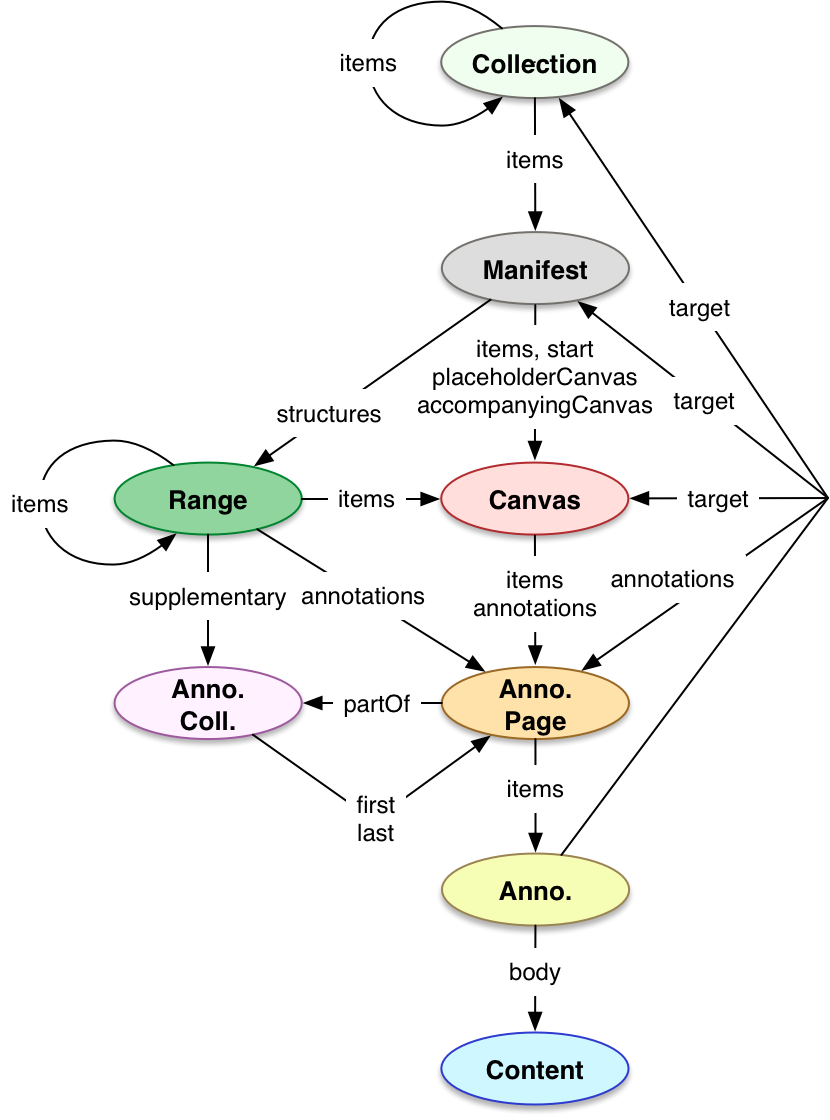
\includegraphics[height=9cm]{figues/modele_donnees_iiif.png}
          \end{center}
		\caption{Structure d'un \man \iiif.\footcite{appleby_presentation_nodate}}

          \label{fig:manifest} \end{figure}

Un canevas peut être considéré comme un espace abstrait sur lequel un
contenu peut être ``peint''. Chaque canevas possède une largeur et une
hauteur qui définissent un espace de coordonnées en deux dimensions,
permettant ainsi de positionner précisément un ou plusieurs
contenus.

Les contenus, servent à remplir un canevas, il s'agit typiquement du
contenu visuel identifié grâce aux \URLs définis par l'\api image.
L'association entre un \texttt{content} et un \texttt{canvas} se réalise à travers une
Annotation, qui peut soit occuper la totalité de l'espace du Canevas,
soit cibler une zone spécifique de celui-ci. Un \texttt{canvas} peut donc aussi
aussi être la cible d'autres types d'annotations (transcription,
commentaires, tags etc.) ciblant des zones particulières au sein de cet
espace de coordonnées.

Cette structure de données permet donc l'alignement des annotations et
des images, y compris si l'utilisateur.rice producteur des annotations est
différent du créateur du \man~; ce qui facilite la collaboration de plusieurs acteurs autour d'un \man produit
par une institution.

Les annotations deviennent à ce titre un élément important et
opérationnel dans le processus de localisation et d'indexation des
coordonnées des diagrammes extraits par le modèle de vision
artificielle. Elles permettent de lier à chaque page de manuscrit et
d'afficher dans un visualiseur la localisation et l'étendue spatiale des objets détectés~; et ce en
récupérant uniquement leurs coordonnées spatiales.

Pour l'entraînement, elles permettent de marquer et de délimiter les
zones spécifiques de l'image où se trouvent les objets que le modèle de
vision artificielle doit identifier~; pour la correction des
prédictions, elles permettent de modifier la tailler et la place d'une
annotation prédite ou d'en créer une nouvelle. La collaboration, enfin,
est essentielle dans les projet impliquant l'annotation à grande échelle
de vérités de terrain.

\hypertarget{avantages-et-limites-du-cadre-iiif}{%
\subsection{Avantages et limites du cadre
IIIF}\label{avantages-et-limites-du-cadre-iiif}}

\emph{Interopérabilité et ouverture de la données}

\iiif garantit l'accessibilité, favorisant la collaboration et l'échange
entre institutions culturelles, universitaires et de recherche,
participant à la visibilité des collections numériques des institutions.
En terme d'interopérabilité, \iiif élimine les barrières techniques entre
différentes plateformes et systèmes, permettant une intégration
transparente des collections d'images. Le cadre et ses protocoles
associés facilitent la recherche et l'analyse d'images en permettant aux
chercheur.ses d'agréger des données provenant de multiples sources et de
les examiner dans un environnement unifié, notamment avec des outils
permettant l'annotation collaborative des images, grâce à un visualiseur comme
Mirador\footnote{https://github.com/ProjectMirador/mirador} ou Universal
Viewer\footnote{https://github.com/UniversalViewer/universalviewer} et à un serveur d'annotations
comme \sas\footnote{\sas est un serveur d'annotations
  \iiif. Il est couplé à la version 2 de Mirador pour la partie cliente
  dédiée à la visualisation des images et à la création des annotations.
  La partie serveur sert à stocker les annotations de façon persistante.
  (https://github.com/glenrobson/SimpleAnnotationServer)}.

\emph{Légèreté}

\begin{kwote}
``{[}\iiif{]} permet de réunir des corpus de sources très diverses, sans
devoir les restocker~; quel que soit le serveur d'où est publié le
document en question, celui-ci peut être visualisé et comparé avec un
document servi par n'importe quelle autre institution publiant des
numérisations \iiif~; ce standard permet aussi, à partir d'une simple
\uri, de récupérer toutes les pages d'un volume particulier dans le bon
ordre, et les métadonnées qui le décrivent.''\footcite[p.6]{champenois_visual_2023}
\end{kwote}   

La solution apportée par l'\api Image répond notamment à la
problématique de l'optimisation du débit de transmission de
l'information lors de la manipulation des éléments graphiques, celle-ci
pouvant être de très haute résolution et de grande taille. En accédant
directement à des extraits spécifiques de l'image d'origine via de
simples transformations d'\URL, l'\api Image permet de la récupérer
uniquement à la taille exacte requise pour une tâche particulière. Cette
flexibilité réduit significativement la quantité de données transférées
sur le réseau, améliorant la fluidité des échanges, essentielle pour les
interfaces interactives et les processus automatisés. L'optimisation du
temps de traitement constitue en effet un enjeux spécifique lié au
traitement de l'image, plus lourde que le texte et plus gourmande en
puissance de calcul.

Ainsi, en donnant accès aux images haute résolution avec des métadonnées
structurées, \iiif facilite l'analyse visuelle et algorithmique des
images. La mise en œuvre de ce protocole standardisé participe donc au
renouvellement du dialogue entre le milieu de la recherche et les
bibliothèques détentrices des données.

Cependant \iiif présente des limites dans son universalité. L'\api
Présentation est le modèle sous-jacent à l'écriture de tout
\emph{\man}. Elle se limite donc à spécifier la sémantique de
présentation, et non la sémantique de description de l'objet lui-même.
Il ne s'agit pas d'un schéma de métadonnées comme Dublin Core ou
\xml \textsc{ead}\footnote{Un schéma de métadonnées est un ensemble de règles qui
  définissent les éléments sémantiques à inclure dans une description
  structurée de données.}, mais d'un format standard pour embarquer les
métadonnées descriptives de l'objet et garantir l'interopérabilité des
\mans entre eux, pour autant un schéma ne porte pas une
sémantique particulière. En pratique, toutes les institutions
n'utilisent pas le modèle de la même manière, ce qui nécessite une
adaptation des développements liés à \iiif pour prendre en compte ces
variations particulières.

\begin{kwote}
``L'application du standard varie ainsi d'une institution à l'autre, sans
altérer le fonctionnement des outils de base de \iiif, mais en provoquant
cependant une déperdition de son universalité pour des projets qui
souhaiteraient développer des outils autour de ces
manifestes.''\footcite[p.25]{norindr_traitement_2023}
\end{kwote}   

À titre d'exemple, alors que le modèle de référence préconise
l'utilisation de la clé \textit{canvases} pour regrouper les images
(Fig. \ref{fig:dresde}), certaines institutions, telles que la
bibliothèque universitaire de Yale (Fig. \ref{fig:yale}),
utilisent \textit{items} à la place, modifiant alors l'arborescence du \man\footcite[p.25]{norindr_traitement_2023}.

          \begin{figure}[H]
          \begin{center}
          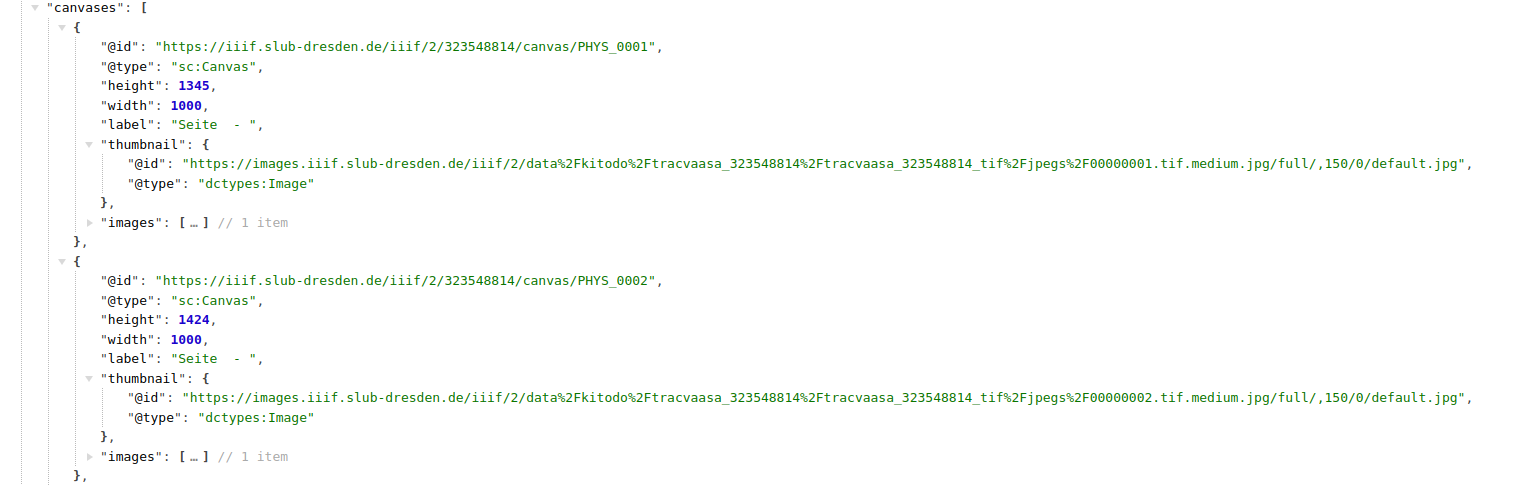
\includegraphics[height=6cm]{figues/dresde_manifest.png}
          \end{center}
          \caption{Usage de \textit{canvases} dans un \man \iiif par Bibliothèque Universitaire de Dresde.}
          \label{fig:dresde} \end{figure}

          \begin{figure}[H]
          \begin{center}
          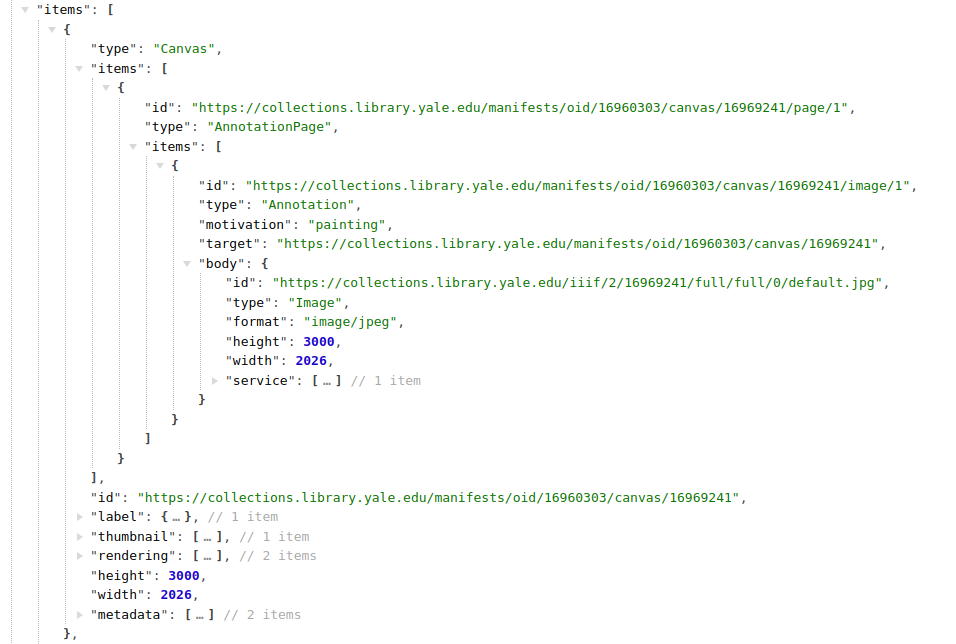
\includegraphics[height=6cm]{figues/yale_manifest.png}
          \end{center}
          \caption{Usage de \textit{items} dans un \man \iiif par Bibliothèque Universitaire de Yale.}
          \label{fig:yale} \end{figure}

Le fichier reste lisible dans un visualiseur, mais la structure du
\man change. Un projet d'exploitation des objets patrimoniaux
reposant sur \iiif, à l'image d'\eida, se doit de connaître les
spécificités propres aux \mans de chaque institution et d'en
adapter le traitement. La récupération et le téléchargement des images
sont gérés par des scripts dédiés qui parsent les \mans
déposés dans l'application. Leur écriture a nécessité une liste des
institutions pourvoyeuses des sources et une connaissance des normes
adoptées pour leur \mans\footnote{\href{https://github.com/Segolene-Albouy/iiif-downloader}{Script for automatic image retrieval from IIIF manifests by Segolène Albouy.}}.
Ces scripts constituent un module indépendant de l'application,
réutilisable et adaptable pour une réutilisation indépendante.

De plus, malgré les avantages évidents qu'elle offre en termes
d'interopérabilité et d'accès aux ressources visuelles l'implémentation
de \iiif n'est pas encore un réflexe systématique et global. Notamment le
monde des musées, hors Amérique du Nord, exploite peu les \api
\iiif\footcite{mallory_iiif_2019}.
Ce contexte fragmente le paysage numérique des ressources culturelles et
complexifie le développement de plateformes telles qu'\aikon. Il est
alors essentiel de prendre en compte la diversité des formats de données
avec lesquels elle pourrait interagir. Ainsi, en intégrant \iiif dans la
plateforme, il est nécessaire d'envisager des mécanismes de
compatibilité avec d'autres formats, en particulier ceux utilisés
couramment dans le domaine des manuscrits numérisés, tels que les
fichiers \textsc{pdf} et les images \jpeg. Cette approche permettra ainsi
d'assurer une grande flexibilité et une interopérabilité optimale,
garantissant la possibilité de traiter une large gamme de sources quel
que soit le format dont dispose l'utilisateur.rice à l'entrée de la chaîne de
traitement.

Ainsi \iiif s'est imposé dans la dernière décennie comme le standard et
une brique technologique essentielle pour décloisonner les collections
numériques des institutions, ouvrant de nouvelles perspectives pour
l'exploration et le traitement du patrimoine visuel à l'échelle
mondiale. Ce protocole contribue à répondre à un enjeu important~:
comment exposer sur le Web une collection patrimoniale de manière
cohérente tout en l'adaptant aux formes diversifiées des pratiques~;
proposant un environnement logiciel gratuit et accessible. Toutefois sa
mise en œuvre généralisée et normalisée est encore en cours. Dans ce
contexte, une chaîne de traitement des sources historiques doit être
conçue de manière à prendre en compte cette réalité, en offrant une
compatibilité avec d'autres formats de données et en s'adaptant aux
spécificités locales des pratiques institutionnelles dans la mise en
œuvre du standard.

\hypertarget{particularite-de-utilisation-de-iiif-au-sein-de-la-plateforme}{%
\subsection{Particularité de l'utilisation de IIIF au sein de la
plateforme}\label{particularite-de-utilisation-de-iiif-au-sein-de-la-plateforme}}

Chaque \textit{record} de \digit dispose d'un \man \iiif spécifique à \eida,
afin de remédier à la variabilité de structure des \mans~: à
la soumission du formulaire d'enregistrement d'un \wit ou d'une \ser, si une \digit a été
ajoutée, les fichiers (déposés au format \textsc{pdf} ou \jpeg, ou bien récupérés à
partir du \man d'une institution) sont téléchargés,
post-traités et renommés. Une vue génère le \man de la
\digit à la demande et il servira de base à l'indexation des
annotations.

L'extraction manuelle ou automatiques de régions d'image entraîne la
création d'une entité \texttt{Regions}, qui dispose de deux \mans pour
faire cohabiter différentes extractions (automatiques et manuelles). Les
annotations issues de l'extraction automatique sont indexées sur un
\man \textit{auto}. Elles sont inscrites \textit{en dur} dans le
\man, ne sont pas indexées dans \sas et ne peuvent pas être
modifiées depuis Mirador. Un \man \textit{v2} est utilisé pour les
annotations réalisées avec \sas, donc effectuées manuellement, ou issues
de la correction des annotations automatiques.

Ces stratégies de développement permettent de palier aux limitations
imposées par le standard \iiif, tout en tirant partie de ses avantages et
de son système d'annotation. Elles permettent aussi plus de flexibilité
dans la méthode d'extraction des objets d'intérêt dans les images, en
autorisant deux types d'annotation, manuelle et automatique.